% Created 2023-01-05 Thu 21:43
% Intended LaTeX compiler: pdflatex
\documentclass[aip, jmp, amsmath, amssymb, nofootinbib]{revtex4-2}
\usepackage[utf8]{inputenc}
\usepackage[T1]{fontenc}
\usepackage{graphicx}
\usepackage{longtable}
\usepackage{wrapfig}
\usepackage{rotating}
\usepackage[normalem]{ulem}
\usepackage{amsmath}
\usepackage{amssymb}
\usepackage{capt-of}
\usepackage{hyperref}
\usepackage[version=4]{mhchem}
\usepackage{listings}
\usepackage{glossaries}
\usepackage[automake]{glossaries-extra}
\usepackage{abstract}%% easy abstract environment (from frontmatter pkg "ltxfront")
\usepackage[export]{adjustbox}%% expanded control over image, minipages, etc
\usepackage{amsthm}%% formal mathematics environments
\usepackage{amsfonts}%% formal math fonts
\usepackage{mathptmx}%% ghostscript/postscript fonts and font loading options
\usepackage{bm}%% bold math
\usepackage{caption}%% full (expands on capt-of) control over appearance of float captions
%\captionsetup{margin=10pt, font=small, labelfont=bf}%% (global preamble, local env)
\usepackage{sidecap}%% control of figure and caption positioning and margin spill
\usepackage{mathtools}%% bugfixing and additional tools for amsmath
\usepackage{upgreek}%% easy lower and uppercase nonitalicized greek letters
\usepackage{soul}%% spaceout and underline macros
\usepackage{xcolor}%% text color macros
\usepackage{natbib}%% required citation engine
%
%% control margin configurations and visualize framing
%% \usepackage[%% Uncomment any one of the following lines to test
%% showframe,
%% scale=0.7, marginratio={1:1, 2:3}, ignoreall, %% default settings
%% text={7in,10in},centering,
%% margin=1.5in,
%% total={6.5in,8.75in}, top=1.2in, left=0.9in, includefoot,
%% height=10in,a5paper,hmargin={3cm,0.8in},
%% ]{geometry}
%
\usepackage{svg}
\svgpath{{/home/panos/Pictures/figs}}
%
\usepackage[acronym,nogroupskip,nonumberlist]{glossaries}
\usepackage[%
stylemods,style=long-short,
]{glossaries-extra}
\makeglossaries
%
%\usepackage[mathlines]{lineno}% Enable numbering of text and display math
%\linenumbers\relax % Commence numbering lines
\newacronym{hap}{HaP}{halide perovskite}
\newacronym{vasp}{VASP}{Vienna Ab initio Simulation Package}
\newacronym{qmml}{QM/ML}{quantum mechanics machine learning}
\newacronym{slme}{SLME}{spectroscopic limited maximum efficiency}
\newacronym{pce}{PCE}{power conversion efficiency}
\newacronym{dft}{DFT}{density functional theory}
\newacronym{gga}{GGA}{generalized gradient approximation}
\newacronym{pbe}{PBE}{Perdew-Burke-Ernzerhof Functional}
\newacronym{hse}{HSE06}{Heyd-Scuseria-Ernzerhof Functional}
\newacronym{ma}{MA}{Methylammonium}
\newacronym{fa}{FA}{Formamidinium}
\newacronym{hap}{HaP}{halide perovskite}
\newacronym{pca}{PCA}{principal component analysis}
\newacronym{tsne}{t-SNE}{t-distributed stochastic neighbor embedding}
\newacronym{umap}{UMAP}{uniform manifold approximation and projection}
\newacronym{gpr}{GPR}{Gaussian Process Regression}
\newacronym{rfr}{RFR}{Random Forest Regression}
\newacronym{sisso}{SISSO}{Sure Independence Screening and Sparsifying Operator}
\newacronym{sqs}{SQS}{special quasi-random structures}
\newacronym{paw}{PAW}{projector augmented wave}
\newacronym{nist}{NIST}{National Institute of Standards and Technology}
\newacronym{pes}{PES}{Potential Energy Surface}
\newacronym{shap}{SHAP}{Shapley Additive Explaination}
\newacronym{gnn}{GNN}{Graph Neural Networks}
\newglossaryentry{cmix}{name=cardinal mixing,description={{Describes perovskite alloys where no more than one of the A, B, or X sites is occupied by multiple possible constituents}}}
\newglossaryentry{prtn}{name=partition,description={{Portion of sample data reserved for a purpose in model development}}}
\newglossaryentry{cv}{name=cross-validation,description={{Method for gathering statistics on the abilities of a model to fit to the parent partition}}}
\newglossaryentry{kfs}{name=K-fold split,description={{Data partition divided into K arbitrary groups for use in cross-validation schemes}}}
\newglossaryentry{gkf}{name=groupwise K-fold,description={{Data partition divided into K-folds where each fold corresponds to a category label}}}
\newglossaryentry{lot}{name=level of theory,description={{Refers to the rank of a [[ACRshort:dft][DFT]] functional in the hierarchy of phenomenological comprehensiveness. A proxy for accuracy.}}}
\newglossaryentry{mp}{name=Materials Project,description={{US Government-led multidisciplinary collaboration founded in 2011 as the Materials Genome Initiative.}}}
\newglossaryentry{ml}{name=machine learning,description={{a science concerned with algorithms which improve their performance with exposure to new data}}}
\newglossaryentry{ft}{name=features,description={{attributes of an observed event or object which might empirically explain the event or object}}}
\newglossaryentry{hp}{name=hyper-parameter,description={{a setting that controls how a learning algorithm works}}}
\newglossaryentry{cl}{name=classical learning,description={{a paradigm of machine learning that is dependent on expert knowledge to extract quality features from samples in a dataset}}}
\newglossaryentry{sm}{name=surrogate model,description={{a representation which attempts to capture as much of the relationship between a domain and a target property as possible}}}
\newglossaryentry{dl}{name=deep learning,description={{a paradigm of machine learning differing from classical learning in that the features of the input data are themselves learned by the algorithm}}}
\newglossaryentry{ls}{name=latent space,description={{a multidimensional abstraction of a problem space. the relationship between coordinates in this space and observation in the real world can be formulated to guarantee the viability of solutions in the abstraction}}}
\newglossaryentry{eva}{name=evolutionary algorithms,description={{a class of nature-inspire algorithms often applied to optimization in high dimensional discontinuous functions}}}
\newglossaryentry{agn}{name=ALIGNN,description={{the Atomistic Line Graph Neural Network considers relative positions of atoms in a crystal as well as the relative angles between bonds by creating two related node and edge graphs and convluting them in a staggered manner together}}}
\newglossaryentry{gp}{name=Gaussian Process,description={{Any function which returns samples from an underlying multivariate normal distribution}}}
\newglossaryentry{fair}{name=FAIR,description={{Findable Accessible Interoperable and Reusable Data}}}
\newglossaryentry{mtl}{name=multi-task learning,description={{A type of machine learning where an algorithm learns multiple functions simultaneously, while exploiting commonalities and differences between the functions}}}
\newglossaryentry{soc}{name=Spin Orbit Coupling,description={{An additional term intended to account for the increased relevance of quantum angular momentum to electromagnetic response in heavy atoms}}}
\author{Panayotis Manganaris}
\date{\today}
\title{}
\hypersetup{
 pdfauthor={Panayotis Manganaris},
 pdftitle={},
 pdfkeywords={},
 pdfsubject={},
 pdfcreator={Emacs 29.0.50 (Org mode 9.5.2)}, 
 pdflang={English}}
\begin{document}

%revtex frontmatter conventions for quick recall via INCLUDE keyword
\title{%
Multi-fidelity Machine Learning Pervoskite Composition vs Band Gap
}
%\thanks{A footnote to the article title}

\author{Panayotis Manganaris}
\author{Jiaqi Yang}
\author{Arun \surname{Mannodi Kanakkithodi}}
\email{amannodi@purdue.edu}
\affiliation{%
School of Materials Engineering,\\
Purdue University, West Lafayette, Indiana 47907, USA
}
\collaboration{Mannodi Research Group}

\date{\today}
\maketitle
%INCLUDE before abstract environment
\begin{abstract}
We report on the details of creating models of halide perovskite properties based on composition and derived
descriptors. The primary objective of these models is to eventually recommend perovskite alloy compositions
corresponding to targeted properties. Here targets are chosen to yield high photovoltaic (PV) performance. So, we focus
on models of the electronic band gap. We leverage the Purdue University nanoHUB, an NSF-funded, Purdue-hosted
computational repository, to host literate reproducible notebooks documenting our model development workflow
\cite{manganaris-2022-mrs-comput}. We thus enable the scientific community to utilize our approach for modeling
performance targets for a wider range of promising compounds.

We explore a variety of machine learning (ML) models for the prediction of Perovskite bandgap. A rigorously optimized
Random Forest Regressor (RFR), a Gaussian Process (GP) Regressor, and a Sure Independent Screening and Sparsifying
Operator\cite{ouyang-2018-sisso} (SISSO) regressor.

Approximately 1500 physical and synthetic records spanning various experimental fidelities and alloy schemes are used in
model development. All experiments are conducted for one of \textasciitilde{}500 perovskite compositions. \textasciitilde{}1400 experiments are
performed computationally using Density Functional Theory (DFT), \textasciitilde{}100 are physical measurements obtained from published
literature\cite{almora-2020-devic-perfor,jiang-2006-predic-lattic,briones-2021-accel-lattic}.

\begin{enumerate}
\item 500 PBE relaxations -> PBE Density of States (DoS) calculation
\item 300 HSE06 relaxations -> HSE06 DoS
\item 300 HSE06 relaxations -> HSE06 + Spin-Orbit Coupling (SOC) DoS
\item 300 PBE relaxations -> HSE06 + SOC DoS
\item 100 experimental band gap measurements
\end{enumerate}

Our models are based primarily on composition information. We implement generic feature extraction by parsing a string
encoding the ABX\textsubscript{3} perovskite formula corresponding to each record. The resulting 14-dimensional composition vector is
easily obtained for experimental and synthetic data alike. This is a sufficient predictor variable, nonetheless we
continue. Secondarily, we also examine 36 additional predictor variables computed as linear combinations of these
compositions and certain elemental properties obtained from the trusted Mendeleev databases \cite{mentel-2014}. Finally,
additional fidelity features are one-hot-encoded with the aim of improving model accuracy. In future work, we anticipate
adding descriptors based on phase and structural information.

We finally compare the band gap models based on this basic 55 dimensional descriptor and models based on an engineered
domain we produced to improve model efficiency, performance, and interpretability.
\end{abstract}
\section*{Introduction}
\label{sec:org3482c4a}
\subsection*{Multi-Fidelity Learning}
\label{sec:orge0a9039}
The state of the art in materials modeling favors \Acrfull{gnn}\cite{chen-2019-graph-networ,choudhary-2021-atomis-line,xie-2018-cryst-graph}
architectures. These \gls{dl} models have sufficient flexibility
to capture the continuous variability in relative positions of
crystals and molecules. They are extremely effective models, but they
are difficult to use with physical materials. Accurately
characterizing structures at a level of atomic granularity cannot be
achieved even with state of the art 3D Electron Tomography
techniques\cite{ercius-2015-elect-tomog}. Yet, characterization of
chemical composition is a well established practice i.e using X-ray
spectroscopy.

Graph convolutional neural networks can power more accurate
structure-target predictions at multiple
fidelities\cite{chen-2020-multi-fidel} by performing \Gls{mtl} (MTL). For instance, this multiple-fidelity machine learning
technique can infer the relationships between more plentiful \ACRshort{pbe} \ACRshort{gga}
data and rarer but more accurate \ACRshort{hse} data based on a shared set of
predicting \gls{ft}. This relationship, if sufficiently general, can
be used to reliably extrapolate from known points on the \ACRshort{pbe} co-domain
to the unknown \ACRshort{hse} co-domain. Of course, while this is implemented
successfully in neural networks, the concept holds for any model
architecture that can simultaneously regress multidimensional targets
which do not need to constitute one rectangular data structure.

Additionally, there are alternative \gls{mtl} approaches
that can be implemented on the domain side. This circumvents the
requirement for flexibility in encoding the co-domain, making it
possible to use a single target regression methods to learn rules for
multiple outcomes that vary depending on a categorical variable
representing the fidelity. In general, the problem of accurately
modeling low availability, high fidelity targets is approached using
MTL to learn regressions on datasets compiled either along X or Y from
measurements taken at multiple \gls{lot}.

Semi-supervised
learning\cite{chapelle-2006-semi-super-learn,lee-2013-pseud-label} is
a competing set of methods achieving similar outcomes.

We will employ the domain-side approach where the largest, lowest
fidelity component of our dataset consists of \acrfull{dft} band gap predictions made at the \acrfull{gga} \acrfull{pbe} \gls{lot}. On
the other end, the smallest and highest fidelity subset of the sample
consists of experimental measurements of physical devices collected
from the literature.

\subsection*{Dataset Overview}
\label{sec:org08a82aa}
\subsubsection*{Perovskite Band Gaps}
\label{sec:org9334c96}
we aim to accurately predict performance-relevant \Acrfull{hap} band gaps which are strongly predictive of photovoltaic
performance\cite{mannodi-kanakkithodi-2019-compr-comput}.

Furthermore, using MTL modeling we aim to predict the experimentally
measured band gaps of compounds that have only been simulated to
date. Our fidelity hierarchy climbs from \ACRshort{dft} simulations performed
using the basic \acrshort{pbe} \acrshort{gga} functional, to results obtained from physical
experiments aggregated in
literature\cite{almora-2020-devic-perfor,kim-2014-cdses-nanow,swanson-2017-co-sublim}
see table \ref{tbl:LoTs}.

While we acknowledge the advantages of \acrshort{gnn}, we aim to express band
gap as functions primarily of the perovskite composition. It is known
this effort is suboptimal especially as the octahedral arrangement of
perovskites is most relevant to their electronic structure,
Nevertheless, a strong understanding of the influence of chemical
composition on performance will continue to be a priority as it is
expected to aid in \hyperref[sec:org007fe94]{inverse design} and in \hyperref[sec:orge549945]{Feature Engineering}.

 
\begin{table}[htbp]
\caption{\label{tbl:LoTs} Density Functionals vs Sample Counts}
\centering
\begin{tabular}{lr}
 & LoT\\
\hline
PBErel & 517\\
HSErel(SOC) & 299\\
HSErel & 297\\
HSE-PBE(SOC) & 244\\
EXP & 44\\
\hline
Total & 1401\\
\end{tabular}
\end{table}

A detailed analysis of this combined hybrid organic-inorganic and
purely inorganic \acrshort{hap} \ACRshort{dft} dataset is covered in a prior article by
\citet{yang-2022-high-throug} and in \hyperref[sec:orgb909428]{DFT Details}.

Naturally, the statistics obtained from each fidelity vary (fig
\ref{fig:bg_dist}). This is the primary challenge we will address with
the categorically dimensioned multi-fidelity models discussed in
\hyperref[sec:org7884545]{Methods}.

 
\begin{figure}[htbp]
\centering
\includesvg[width=300pt]{./.ob-jupyter/d2e07289c9acdbf81dae438b7d5241ccb00224a8}
\caption{\label{fig:bg_dist} Variability in band gap per level of theory}
\end{figure}

\subsubsection*{Sampling}
\label{sec:org02dfb96}
The simulations for each \gls{lot} are performed on some number
of members to a fixed subset of the total 37785 compositions that can
be combinatorially generated in a 2x2x2 perovskite supercell when
allowing \emph{at most} single-site alloying with our 14 constituent
candidates for 3 sites (table \ref{tbl:site_tbl}).

\begin{table}[htbp]
\caption{\label{tbl:site_tbl} ABX\textsubscript{3} Chemical Domain}
\centering
\begin{tabular}{l|llllll}
A-site & \ACRshort{ma} & \ACRshort{fa} & Cs & Rb & K & \\
B-site & Pb & Sn & Ge & Ba & Sr & Ca\\
X-site & I & Br & Cl &  &  & \\
\end{tabular}
\end{table}

Within this sample space, we try to maintain a balance in the share of
samples that represent each one of the "\gls{cmix}"
categories. Additionally, within each mix we try to maintain a
reasonable balance of purely inorganic samples versus hybrid
organic-inorganic samples. See figure \ref{fig:lot_mix_org}. See \hyperref[sec:org7884545]{Methods}
for details on how these categories were utilized in model
development.

The design of this dataset provides an opportunity to assess the
ability of our models to extrapolate with respect to alloying scheme
as well as \gls{lot}. It also provides an opportunity to
investigate the statistical impact of constituent compounds on
perovskite property prediction. See \hyperref[sec:org9df7bc6]{Results and Discussion}.

 
\begin{figure}[htbp]
\centering
\includesvg[inkscapeformat=png, inkscapedpi=300,width=300pt]{./.ob-jupyter/714175a3d13e3c523962f378572a20cc21500c4d}
\caption{\label{fig:lot_mix_org} Share by count of total data apportioned from each experimental subcategory}
\end{figure}

\subsection*{Model Optimization}
\label{sec:orge5c1912}
The rigorous \gls{hp} Optimization (HPO) of any feature
engineering and modeling pipeline is a problem discussed extensively
in the literature. HPO approaches can be broadly separated into
exhaustive and efficient optimization strategies
\cite{yang-2020-hyper-optim}. We use a two-stage procedure for
selecting the best model parameters.

The first stage is an exhaustive grid-search over diversely sampled
parameter space. Each combination of parameters instantiates a model
which is then fit to each of a set of stratified training subsets
generated by a K=3 \gls{kfs} \gls{cv} strategy. Every
fitted model is subsequently tested against the \gls{cv} test
sets and a suite of regression scoring metrics are applied to each
member category simultaneously using a custom scikit-learn score
adapter\footnote{\url{https://github.com/PanayotisManganaris/yogi}\label{orgda4b78a}}.

The grid search is then narrowed to a high performance quadrant of the
search space by the model evaluator based on recommendations made by a
simple entropy minimization algorithm\textsuperscript{\ref{orgda4b78a}}.

In general, the recommended grid quickly eliminates under-performing
settings based on the sample probability of a setting appearing in a
set of finalists according to the scoring rankings. The selection
score is additionally influenced by a weighted sum of the scoring
ranks allowing for considerably tuning the selection criterion.  For
best results, a few different grid spaces should be explored to
corroborate eliminations.

After the recommendation is made, the granularity of the grid is
increased in the remaining ambiguous parameters and the process is
repeated. In general, no more than 2 or 3 exhaustive searches are
needed over a given set of grids.

Past this point, continuously variable hyper parameters can be
individually optimized using validation curves.

\section*{Methods}
\label{sec:org7884545}
\subsection*{DFT Details}
\label{sec:orgb909428}
The largest subdivision of 1400 compounds correspond to a series of
optoelectronic \acrshort{dft} simulations. The simulated experiments are
performed on some subset (table \ref{tbl:LoTs}) of \textasciitilde{}500, exclusively
pseudo-cubic, ABX\textsubscript{3} supercells obtained by geometry optimization of
modified structure files \cite{pilania-2016-machin-learn} originally
obtained from the Computational Materials Repository\footnote{\url{https://cmr.fysik.dtu.dk/}}. Each cell
demonstrates an \acrshort{sqs} mixed composition at none or one of each of the A,
B, or X sites.

Each relaxed structure is made in two ways. Once with the \acrshort{pbe} \acrshort{gga}
functional and once with the \acrshort{hse} functional. Band gaps are obtained
using a static band structure calculation performed at the same and at
higher \gls{lot}.

The chosen functionals each offer strengths and weaknesses. \acrshort{pbe} is
inexpensive but typically underestimates band gaps. \acrshort{hse} is orders of
magnitude more expensive and may fail to converge structure
relaxations but tends to be more trustworthy for electronic structure
properties. HSE06 on PBE relaxation attempts to mitigate the
disadvantages of each individually. The use of \gls{soc}
helps to better electronic properties simulation in compounds
containing Lead.

\subsection*{Featurization of Chemistries}
\label{sec:org6fe3a2d}
For \(\alpha\) total A-site constituents represented in the whole
database, \(\beta\) total B-site constituents, and \(\gamma\) total X-site
constituents, we provide a Python tool\footnote{\url{https://github.com/PanayotisManganaris/cmcl}\label{org9f1ad34}} which robustly coverts
the composition string of each data point into a \(\alpha + \beta +
\gamma\) dimensional composition vector. In the case of our dataset
description\cite{yang-2022-high-throug} \(\alpha + \beta + \gamma =
14\). 

\lstset{language=jupyter-python,label= ,caption={An example of the cmcl "ft" feature accessor},captionpos=b,numbers=none}
\begin{lstlisting}
subset = [883,886]
df = Y.Formula[subset].to_frame().ft.comp()
df.index = Y.Formula[subset]
print(df)
\end{lstlisting}

\begin{verbatim}
                     MA   FA  Pb     I    Br
Formula                                     
MA0.7FA0.3PbI3      0.7  0.3   1  3.00   NaN
MAPb(I0.41Br0.59)3  1.0  NaN   1  1.23  1.77
\end{verbatim}

This is naturally a sparse, relatively high dimensional
descriptor. With any growth in the composition space it becomes
sparser. This descriptor has been shown to be effective for
interpolating the properties of irregularly mixed large
supercells\cite{mannodi-kanakkithodi-2022-data-driven}, However, a
spare descriptor is generally bad for extrapolative
modeling\cite{ghiringhelli-2015-big-data}. When extrapolation is the
aim, continuously distributed, unique, and linearly independent
features are much more reliable\cite{lux-2020-inter-spars}. Our
attempts to provide a domain with these characteristics results in the
following raw feature space.

\begin{itemize}
\item 14 sparse composition vectors extracted from chemical formula
\begin{itemize}
\item generated using cmcl\textsuperscript{\ref{org9f1ad34}}
\item see \hyperref[sec:orgc3205dc]{Predictor Variables}
\end{itemize}
\item 36 dense site-averaged property space
\begin{itemize}
\item computed as a linear combination of composition vectors and
measured elemental properties\cite{mentel-2014}
\item see \hyperref[sec:orgc3205dc]{Predictor Variables}
\end{itemize}
\item 5 categorical dimensions one-hot-encoding \gls{lot}.
\begin{itemize}
\item this provides the domain-side categorical axis for \gls{mtl}
\item see table \ref{tbl:LoTs}
\end{itemize}
\end{itemize}

\subsection*{Machine Learning Algorithms and Parameter Optimization}
\label{sec:org5b69c0a}
We train \acrshort{rfr} and \acrshort{gpr} models of band gap on the union of predictor
\gls{ft} previously discussed. The \acrshort{rfr} is a flexible nonlinear model,
the \acrshort{gpr} a principled linear model. We hope \Acrfull{shap} analysis of the models will lend insight to the
average physical impacts of 1) site-specific alloying and 2) using
organic molecules in the Perovskite superstructure.  Model development
and feature extraction is performed using Python and
SciKit-Learn\cite{pedregosa-2011-scikit-learn} v1.2.

We are careful to maintain the diversity of mixing types and
hybrid-organic/inorganic samples within each fidelity subset. We
expect this will help to ensure the models learn relationships between
fidelities, not differences in alloy scheme or constituency
distributions within each fidelity.

Each model architecture is rigorously optimized with regard to both 1)
generality over the domains of Perovskite compositions and
site-averaged constituent properties and 2) generality over the domain
of alloy classifications.

In order to monitor for possible categorical biases effecting
regressions, nine metrics are used to evaluate the performance of each
model over all alloy types at every stage of the hyper-parameter
optimization. This is done simultaneously, only models that perform
uniformly well on all alloy types are selected.

We expect perovskites of a given alloy class and of a given
hybrid-organic/inorganic status will perform significantly differently
with respect to a particular application compared to perovskites of a
another class or status. We attempt to make models that reasonably
explain this high entropy mixing diversity by utilizing the \gls{cmix} represented in our sample.

We do this by training each model using two test/train splits. First,
the optimal model parameters are chosen for their performance under a
random split. A minimum of 3-fold cross-validation is performed for
every set of model parameters that is considered (See \hyperref[sec:org8a7016b]{Learning Curves}). Finally, the optimized model's ability to extrapolate is
tested by training/testing on splits determined with a \gls{gkf} splitting strategy.

Two separate cross validation schemes are employed at each stage of
the design process. First, the sample set is shuffled once and split
to mitigate the models tendency to fit on sample order, then,
stratified K-folds are generated in manner consistent with the types
of each sample. The regressor is then trained on the subsets of each
class. Its ability to extrapolate is independently metered on each
validation fold consisting of members of the other classes.

Second, the ability for a model trained on samples belonging to one
class/status to extrapolate to samples of another class/status is
tested as well. The samples again are shuffled and split. then the
training set is separated using a grouping K-fold split strategy.

A final best model is instantiated using the overall best performing
parameters. These models are finally validated against the test sets
originally split off from the sample in both their extrapolative
ability and consistency across groups.

This procedure in demonstrated in an online notebook by
\citet{manganaris-2022-mrs-comput} hosted on the Purdue NanoHUB.

\subsection*{Feature Engineering}
\label{sec:orge549945}
There has been success in creating analytical expressions for
perovskite properties, particularly lattice
parameters\cite{jiang-2006-predic-lattic}. In an attempt to find an
analytical predictor for band gap we employ the \Acrfull{sisso}\cite{ouyang-2018-sisso}.

SIS\footnote{\url{https://github.com/rouyang2017/SISSO}} is a powerful application of compressed
sensing\cite{ghiringhelli-2017-learn-physic}. The SIS operator is a
potent dimensionality reduction technique. It does not perform any
mathematical decomposition but instead picks existent dimensions that
begin to approximate an orthogonal basis it outperforms
CUR\cite{ray-2021-various-dimen,hamm-2019-cur-decom} decomposition by
functioning effectively in extremely high rank vector spaces. This is
accomplished by posing the decomposition as a compressed sensing
problem in the correlation metric space. We provide a Sci-Kit Learn

It allows the program to effectively find candidates for a linearly
independent basis in a vector space of immense size. unlike legacy
techniques, e.g. LASSO, it does not suffer when \gls{ft} are
correlated\cite{tibshirani-1996-regres-shrin,gauraha-2018-introd-to-lasso}. This
allows for it to be used in performing a brute force search of a
super-space generated by combinatorial operations on the raw \hyperref[sec:orgc3205dc]{Predictor Variables}.

The Sparsifying Operator finds members of the resulting basis set
which correlate with the target co-domain. it does this by creating a
sparsified linear model, similar again to a LASSO. This process
produces an analytic model of the target property, which is easy to
interpret and can even be constrained for consistent combination of
dimension units.

Subsequent applications of the SIS operator to the residuals of this
model are a clever interrogation of error\cite{mayo-1998-error-growt}
yielding more orthogonal basis sets that can be incorporated into the
model

\acrshort{sisso} is run for our dataset on the same partitioning scheme used by
the previous models via an scikit-learn
compliant\cite{buitinck-2013-api} interface\footnote{\url{https://github.com/PanayotisManganaris/pysisso}} extensively modified
from the original Matgenix\footnote{\url{https://github.com/Matgenix/pysisso}} code. Additionally, the algorithm is
informed of \gls{ft} units so that it is restricted to meaningful
linear combinations. SIS \gls{ft} complexity is restricted to a
maximum of 3 operations primarily to encourage parsimonious
descriptions. The available operation set is outlined in table
\ref{tbl:ops}.

\begin{table}[htbp]
\caption{\label{tbl:ops} operations for formation of combinatorial super-space}
\centering
\begin{tabular}{ll}
Binary (dimensional) & Unary (dimensionless)\\
\hline
addition & reciprocation\\
subtraction & power 2\\
multiplication & power 3\\
division & natural logarithm\\
 & exponentiation\\
 & root 2\\
\end{tabular}
\end{table}

\section*{Results and Discussion}
\label{sec:org9df7bc6}
\subsection*{Best Models on Raw Domain}
\label{sec:org73a625b}
 
\begin{multicol}
\centering
\includesvg[inkscapeformat=png, inkscapedpi=300,width=450pt]{./.ob-jupyter/e8d56a58c17c3b333f96a8fa83097eab4eca15ee}
\caption{\label{fig:pairplots} Multi-fidelity model predictions vs Experimental values}
\end{multicol}

The exhaustively optimized models are obviously high performing (Table
\ref{tbl:rawLoTscores}). The \acrshort{rfr} \gls{hp} are listed in \hyperref[sec:org8c0870f]{HPO Summary Tables} (Table \ref{tbl:rfrHPO}). The \acrshort{gpr} model is tried with
multiple kernels. Ultimately, the best is a non stationary Matern
kernel with \(\nu = \frac{3}{2}\).

\subsection*{SHAP Analysis of Domain}
\label{sec:orga571974}
\begin{figure}[htbp]
\centering
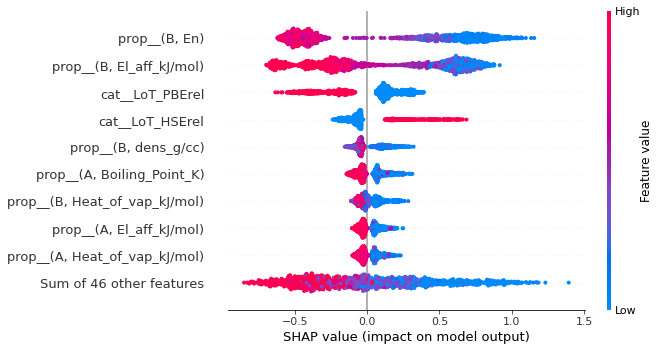
\includegraphics[width=450pt]{./RFR/.ob-jupyter/704d3204752bc52a936aeb9d96e45380512c8c3d.png}
\caption{\label{fig:rfrSHAP} Random Forest Regression Band Gap SHAP Values}
\end{figure}

\acrshort{shap} scores are computed automatically for every dimension of every
sample in the domain. The sum of \acrshort{shap} scores computed for each
predictor variable of a sample is the model's prediction for that
sample\cite{lundberg-2017-unified-approac}.

Figures \ref{fig:rfrSHAP} and \ref{fig:gprSHAP} show the aggregated score
results. Within each figure, \gls{ft} are ranked by overall value on
the y-axis. The x-axis shows the \acrshort{shap} score for each point. The points
are shaped in a violin plot to show the distribution of effects the
presence of the given feature can have. Finally, on the z-axis,
feature value gives a sense of how often the feature is a relatively
minor contributor to a prediction.

For instance, in figure \ref{fig:rfrSHAP}, the B-site Electronegativity
is fairly often a strongly positive contributor to the \acrshort{rfr}
prediction. However, almost always in this case it is out-contributed
by other \gls{ft} -- it does not mostly determine the result but it is
still valuable. On the contrary, when it is a strongly negative
contributor it effectively determines the result, the model uses small
positive contributions from other features to claw back up to a
positive valued band gap.

\begin{figure}[htbp]
\centering
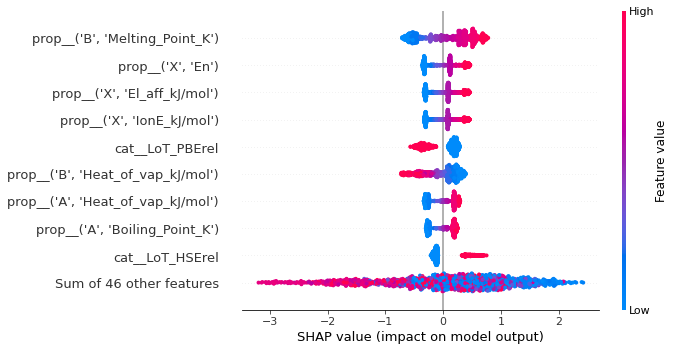
\includegraphics[width=450pt]{./GPR/.ob-jupyter/df8f4cdfbd4884fe978d0b0dc85e13e95137248c.png}
\caption{\label{fig:gprSHAP} Gaussian Process Regression Band Gap SHAP Values}
\end{figure}

These \acrshort{shap} scores can be used to gain insights into the contributions
of site members and site member properties to the perovskite band
gap.

\subsection*{Comparing Feature Usefulness to Raw Correlations}
\label{sec:org290554b}
It is interesting to see how models make use of features in light of
basic bi-variate correlations. The only \gls{ft} that correlate
strongly with band gap are illustrated in figure \ref{fig:rpear}.

 
\begin{figure}[htbp]
\centering
\includesvg[inkscapeformat=png, inkscapedpi=300,width=200pt]{./.ob-jupyter/bee19f4a89b8480a3d67cc87af798e711d963581}
\caption{\label{fig:rpear} raw features with (\(|p|>0.5\)) against band gap}
\end{figure}

\subsection*{SISSO Model and Incidental Engineered Features}
\label{sec:org5194694}
The \Acrfull{sisso}
\cite{ouyang-2018-sisso,ghiringhelli-2017-learn-physic} is a specific
combination of multiple data mining techniques chained together
resulting in a symbolically expressed regression model.

The best model for band gap returned by 5 trials of SISSO involves 3
SIS \gls{ft} and has an unremarkable RMSE of 0.4625 eV, barely
outperforming an OLS regression on 55 dimensions (see Table
\ref{tbl:rawLoTscores}). It is expressed in equation
\ref{eq:bgexp}. Notably, while the units of the expression do not match
the units of band gap as measured (target units are unknown to the
algorithm), they are still energy units.

\begin{align}
\label{eq:bgexp}
bg\mbox{ [eV]} = 1.752075117(&(X;\mbox{Electronegativity}*A;\mbox{Heat of Fusion})\\ \nonumber
                &-(B;\mbox{Ionization Energy}+B;\mbox{Electron affinity}))\\ \nonumber
- 0.5759612116(&B;\ce{Sn}+X;\mbox{Z}-\mbox{HSErel}-\mbox{PBErel})\\ \nonumber
+ 1.074246385(&(A;\mbox{Electronegativity}-B;\ce{Ca})\\ \nonumber
             &\times(B;\mbox{Heat of Vaporization}-X;\mbox{Ionization Energy}))\\ \nonumber
+ 5.254074603 &\mbox{ [kJ/mol]}
\end{align}

\begin{table}[htbp]
\caption{\label{tbl:rawLoTscores} RMSE of models on raw domain calculated per LoT subset}
\centering
\begin{tabular}{lrrrr}
Score Categories & GPR & RFR & Linear OLS & SISSO\\
\hline
rmse & 0.258387 & 0.134671 & 0.499558 & 0.474754\\
rmse EXP & 0.157147 & 0.188727 & 0.307186 & 0.330080\\
rmse PBE & 0.204187 & 0.102778 & 0.472430 & 0.395827\\
rmse HSE & 0.337971 & 0.170726 & 0.558077 & 0.519706\\
rmse HSE(SOC) & 0.275642 & 0.102896 & 0.535087 & 0.572644\\
rmse HSE-PBE(SOC) & 0.245003 & 0.162380 & 0.466364 & 0.470758\\
\end{tabular}
\end{table}

Computing and combining more than 3 SIS \gls{ft} is not rewarding of
the computational expense. Residuals are increasingly uncorrelated
with the generated SIS \gls{ft} and model accuracy gains do not
outstrip complexity. However, in the process of creating Equation
\ref{eq:bgexp}, 150 SIS predictor variables were determined and
recorded. 50 primary predictors, 50 first residual predictors, and 50
second residual predictors. These can serve as a high quality,
introspective domain for the other architectures to fit on.

We set the aim of decreasing \(\mathcal{O}(n^3)\) computational
expense of \acrshort{gpr} by \(\approx\)10 times. So, we aim to take 20 highly
correlated \gls{ft} (slightly less than one half the number used by
prior models) from these SIS subspaces. We expect this to solve the
problems inherent to the raw \hyperref[sec:org6fe3a2d]{Featurization of Chemistries}

Computing \ACRshort{gpr} in conjunction with SIS \gls{ft}, we can create
extrapolative models on a much more continuous domain. Using \ACRshort{gpr} on
the SIS subspaces also leverages SISSO's explicability while obtaining
uncertainty estimates, which is helpful for our inverse design
ambitions.

\subsection*{Best Models on Engineered Domain}
\label{sec:org546cba0}
\section*{Future Work}
\label{sec:org007fe94}
\subsection*{Data Science and Materials Engineering}
\label{sec:orgd5e3b3f}
This has been an exercise in explaining a key performance determining
property of \Acrfull{hap} using only composition
information. Of course, the point of this basic approach is to enable
experimental data to be more easily integrated into predictive models
than is possible with graph-based Convolutional Neural Networks.

Naturally, this invites effort to incorporate much mode experimental
data. Some sources by
\citet{jacobsson-2021-open-acces,briones-2021-accel-lattic} are prime
for consideration.

Notably, in this work, we assume that all compounds involved in this
model manifest in the same pseudo-cubic phase for
simplicity. Unfortunately, this is not nearly accurate to reality. Our
experience with experimental collaborators indicates effective
application of these models to practical synthesis requires that
realistic phase information is somehow incorporated. Ideally this
information can be encoded in an interoperable way for both
computational and physical experiments.

Finally, these models have iterated on prior composition-only models
of band-gap for inverse
design\cite{mannodi-kanakkithodi-2022-data-driven}. They achieve nearly
50\% improvement in accuracy by leveraging more data and, in the case
of models on the engineered domain, higher quality predictor
variables. Using the best performing model and an accompanying model
designed to predict stability in an improved, data-driven perovskites
design framework follows naturally.  In particular, the \ACRshort{gpr} should
drive an active learning approach.

An ongoing goal will be to grow a database of experimentally examined
perovskite photovoltaic prototypes with well defined structures.

\subsection*{Software Tools}
\label{sec:org050f82f}
A couple of libraries are in development for easing the aggregation,
accessing, sharing, and analysis of this data. The current database is
packaged in "cmcl" at \url{http://github.com/PanayotisManganaris/cmcl} under
the tag v0.1.5. In this early stage of development, cmcl strives to
provide an "inquisitive" interface to perovskite composition feature
computers in the style of the pandas API. At its current stage, it has
been useful for extracting composition vectors from the formula
strings identifying each compound.

A library of model evaluation tools to assist with exhaustive grid
search is being maintained in the "yogi" repository at
\url{http://github.com/PanayotisManganaris/yogi}

\section*{}
\label{sec:orgaeda7a2}
\pagebreak
\bibliographystyle{aipnum4-2}
\bibliography{../../../org/bibliotex/bibliotex}
\printglossaries

\section*{Appendix}
\label{sec:orgb413660}
\subsection*{Predictor Variables}
\label{sec:orgc3205dc}
 
\begin{figure}[htbp]
\centering
\includesvg[width=450pt]{./.ob-jupyter/c8a78405cb1cda4d5ce76da6352ea746d4ae9f0c}
\caption{Normalized Distribution of A-site Constituents}
\end{figure}

 
\begin{figure}[htbp]
\centering
\includesvg[width=450pt]{./.ob-jupyter/5026578029e767c7954e424ba9580ae9c7672b60}
\caption{Normalized Distribution of B-site Constituents}
\end{figure}

 
\begin{figure}[htbp]
\centering
\includesvg[width=450pt]{./.ob-jupyter/2407b4c5d1b25479ab1ba73dee37ae53f46fd8e2}
\caption{Normalized Distribution of X-site Constituents}
\end{figure}

Site-averaged elemental properties are derived from the composition
vectors. Twelve properties are computed per \(\ch{ABX_3}\)
constituent. These are much denser distributions.
\begin{enumerate}
\item Ionic Radius
\item Boiling Temperature
\item Melting Temperature
\item Density
\item Atomic Weight
\item Electron Affinity
\item Ionization Energy
\item Heat of Fusion
\item Heat of Vaporization
\item Electronegativity
\item Atomic Number
\item Period
\end{enumerate}

 
\begin{figure}[htbp]
\centering
\includesvg[width=450pt]{./.ob-jupyter/693a93309ca0810b0ef94d8b01d1dea58c2b18c5}
\caption{Distributions of Mean A-Site Properties}
\end{figure}

 
\begin{figure}[htbp]
\centering
\includesvg[width=450pt]{./.ob-jupyter/a4faa833409744e179146795cdd3b0f60f5c3db2}
\caption{Distributions of Mean B-Site Properties}
\end{figure}

 
\begin{figure}[htbp]
\centering
\includesvg[width=450pt]{./.ob-jupyter/c46d84697e84e3f3a88d840460eb128428d81cc3}
\caption{Distributions of Mean X-Site Properties}
\end{figure}

\subsection*{Learning Curves}
\label{sec:org8a7016b}
Learning curves are computed for each scorer. Notice that the error
metrics are negated for consistency with the R\textsuperscript{2} and ev scores; the
greater the number, the better the model performs.

Cross-validation within the training set is the only way of checking
the generality of models during the grid search. Identifying the
validation split size is necessary to obtain an understanding of how
much data is needed to train a model that can generalize.

More data offers better chances. However, the smaller the split, the
longer and more expensive the loop training becomes, e.g. 10-fold
splits makes for 10 sample scores at each partition size. Meaning, 90\%
of the training set is used for actual training and the remaining 10\%
is used for validation and this is repeated 10 times.

Shuffling is performed prior to generating each fold. The shuffle is
seeded with a deterministic random state to ensure scores are
comparable across partition size

\subsection*{HPO Summary Tables}
\label{sec:org8c0870f}
\subsubsection*{Random Forest Pipeline Control Parameters}
\label{sec:orgd671560}

\begin{table}[htbp]
\caption{\label{tbl:rfrHPO} Select hyper-parameters from exhaustive search of 10368 models}
\centering
\begin{tabular}{lll}
 & Search Space & Selected Space\\
\hline
normalizer\_\textsubscript{norm} & [l1, l2, max] & [l2]\\
bootstrap & [True] & [True]\\
ccp\textsubscript{alpha} & [0.0, 0.002] & [0.0]\\
criterion & [squared\textsubscript{error}, absolute\textsubscript{error}, poisson] & [absolute\textsubscript{error}]\\
max\textsubscript{depth} & [25, 20] & [20]\\
max\textsubscript{features} & [auto, 3, 5] & [1.0]\\
max\textsubscript{leaf}\textsubscript{nodes} & [700, 800] & [750]\\
max\textsubscript{samples} & [0.9, 0.6, 0.3] & [0.9]\\
min\textsubscript{impurity}\textsubscript{decrease} & [0.0, 0.3] & [0.0]\\
min\textsubscript{samples}\textsubscript{leaf} & [1] & [1]\\
min\textsubscript{samples}\textsubscript{split} & [2, 5] & [2]\\
min\textsubscript{weight}\textsubscript{fraction}\textsubscript{leaf} & [0.0] & [0.0]\\
n\textsubscript{estimators} & [20, 50, 100] & [150]\\
n\textsubscript{jobs} & [4] & [4]\\
oob\textsubscript{score} & [True] & [True]\\
random\textsubscript{state} & [None] & [None]\\
verbose & [0] & [0]\\
warm\textsubscript{start} & [False] & [False]\\
\end{tabular}
\end{table}
\end{document}